--- from theory section

\iffalse
If a subset of the strings in $S$ are mutually meshable, the corresponding set of nodes in the meshing graph form a clique.  If we choose some clique cover on the graph, this is equivalent to a legal meshing of strings in the string multi-set (where trivial cliques of size one represent unmeshed strings).  The number of cliques is exactly equal to the corresponding number of meshes and unmeshed nodes, which is precisely the quantity we are trying to minimize.
\fi


\iffalse
, m = 1000$, we expect to have fewer than two triangles in the meshing graph.

hen the probability $s_i$ meshes with $s_j$ is
\[
p_{ij}={{n-b_i \choose b_j}} \big / {{n \choose b_j}}
\]
and if all edges were independent the probability that all three strings mesh would be $p_{12}p_{23}p_{13}$ which is actually high that

and therefore if every mesh was independent, the probability that $s_1,s_2,s_3$ form a triangle in the meshing graph would be $p_{12}p_{23}p{}$

The allocation procedure described in \S~\ref{sec:allocation-algorithm} allocates objects uniformly at random from the free space in a span. It is reasonable to assume that each bit in each string is 1 independently with probability $p$ proportional to the global average occupancy.  However, at times, this makes our analysis less straightforward.  Therefore, we typically first assume that all strings have exactly equal occupancies, and then argue experimentally and analytically that similar results hold for the independent case.

\subsubsection{Assume all spans equally full}
Assume that each string in $S$ has exactly $n$ ones.  In other words, each string has occupancy $n$.  Then the probability of an edge in the meshing graph is $q = {{{b-n}\choose{n}}}/{{{b}\choose{n}}}$.  The degree of each node is \texttildelow $Bin \lp m-1,q \rp$.  While edges are two-way independent, they are not necessarily three-way independent --- specifically, possible edges in a cycle are not independent of each other.

\subsubsection{Assume bits 1 independently}
Assume that each bit in each string is 1 independently with probability p.  Then the occupancy of each string is a random variable $n$ \texttildelow $Bin \lp b, p \rp$ with mean $bp$.  The probability of an edge in the meshing graph is $q = \lp 1-p^2 \rp ^b$.  Unlike the constant
occupancy case, we cannot say that edges are two-way independent; possible edges connected by any path are not independent of each other.

\paragraph{Clique Cover and Max Matching}
\fi


\iffalse
We have established that while the meshing problem has a polynomial time algorithm, its runtime is not practical.  Worse, , suggesting that considering MCC at all is impractical.

Luckily, approximating MCC may not be necessary, even if we desire near-optimal meshings. We can simply compute the maximum matching (a much easier computational task) instead.  This is because triangles (and therefore larger cliques) are rare in meshing graphs.  In a graph with no triangles, the min clique cover problem degenerates to the maximum matching problem.  In a graph with few triangles (and therefore no larger cliques with high probability), the min clique cover will differ by the maximum matching by at most 1 for every triangle.

Intuitively, an edge in a meshing graph can be thought of as an indicator of \textit{difference} between two strings.  If strings $\str_1$ and $\str_2$ mesh, and $\str_2$ and $\str_3$ mesh, then $\str_1$ and $\str_3$ are both different from $\str_2$, which means they are more likely to be the same (and therefore not mesh).


More rigorously, in the constant occupancy $r$ case, the probability of a triangle between any three nodes is $$\frac{{{b-r}\choose{r}}}{{{b}\choose{r}}}\frac{{{b-2r}\choose{r}}}{{{b}\choose{r}}}$$ so the expected number of triangles in the entire graph is $${{n}\choose{3}}\frac{{{b-r}\choose{r}}}{{{b}\choose{r}}}\frac{{{b-2r}\choose{r}}}{{{b}\choose{r}}}$$.

In most practical cases, we will not be interested in meshing strings with low occupancy --- it is often better just to wait until the last objects on these spans are freed.  For higher occupancies, the expected number of triangles is quite low.  For instance, if $b = 32, r = 10, m = 1000$, we expect to have fewer than two triangles in the meshing graph.

\begin{comment}
  We have experimentally verified this result by generating many random
constant occupancy graphs and, for each graph, compared the size of the
maximum matching to the size of a greedy (non-optimal) solution for
min clique cover. The results are summarized in the Appendix.
\end{comment}

\fi

\iffalse
\begin{figure}[!t]
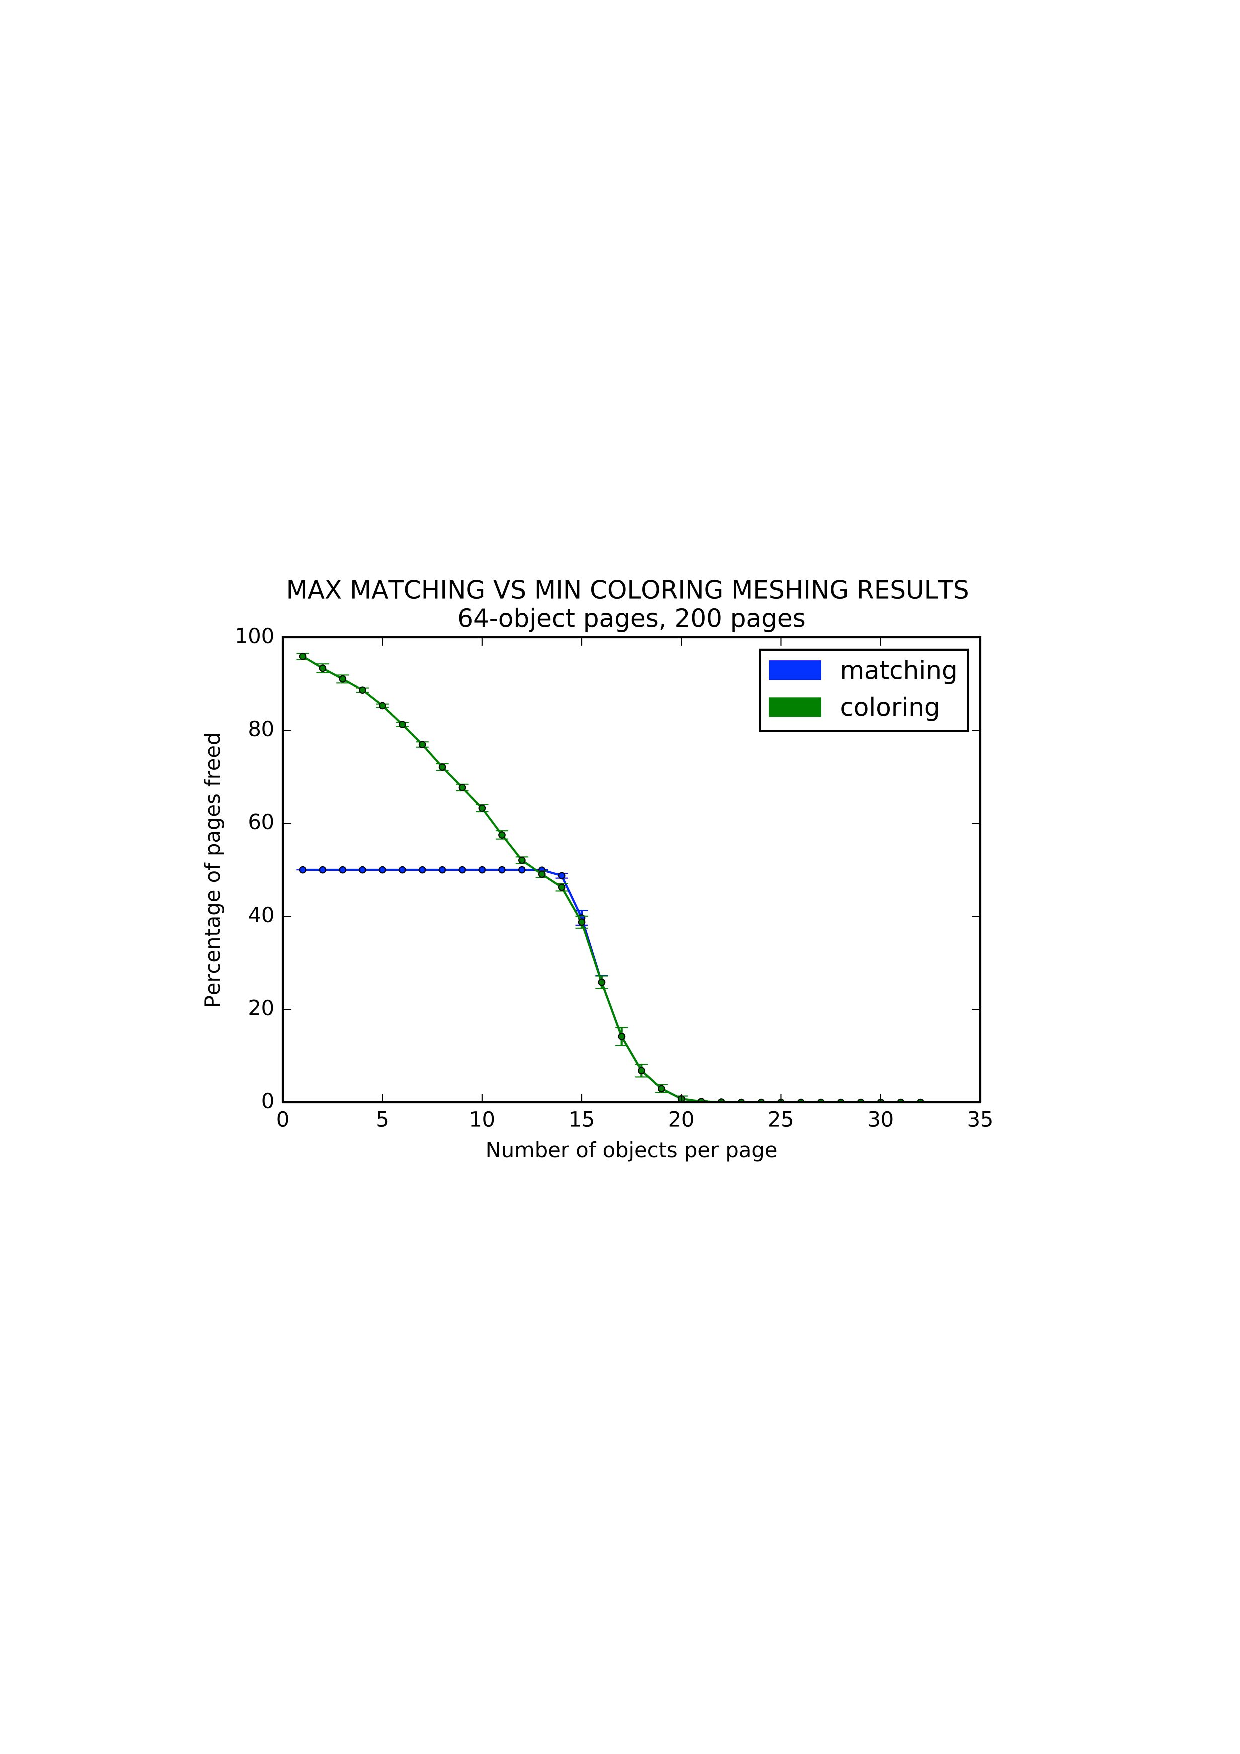
\includegraphics[scale = .5]{figures/comparison.pdf}
\centering
\caption{Average values for max matching and min clique cover on randomly generated graphs.  Ten graphs were generated for each occupancy.}
\end{figure}

For these parameters, the $n = 10$ to $n = 17$ range is where we are most likely to try meshing.  See the "Thresholds" section below for more detail on how this is determined.\\
\fi

\iffalse
For independent bit graphs, the probability that any three nodes form a clique is $$\lp \lp 1-p\rp ^3 - 3\lp 1-p\rp ^2p\rp ^b$$ so the expected number of triangles for the entire graph is $${{m}\choose{3}}\lp \lp 1-p\rp ^3 - 3\lp 1-p\rp ^2p\rp ^b$$.

This is significantly larger than the constant occupancy case for similar expected occupancy.  For $p = n/b = 10/32, m = 1000$, the expected number of triangles is roughly 36,000.
\fi
\iffalse
While constant occupancy graphs are fairly regular,
independent bit graphs may not be. Since strings have different
occupancies, nodes which correspond to strings with relatively low
occupancy will tend to have significantly higher degree than other
nodes in the graph.  Meanwhile, other nodes may have strings with high
occupancy, and therefore only have a few edges (probably with
low-occupancy nodes).  So while there are many triangles, when the
graph is sparse enough, even meshing cliques of size 3 and 4 will
likely ``abandon'' adjacent high-occupancy nodes, one of which could
have been matched with the high degree node to yield the same number
of releases. So, we still expect finding the maximum matching to be
good enough. This behavior is verified experimentally in the Appendix.
\fi


\iffalse
\begin{figure}[h]
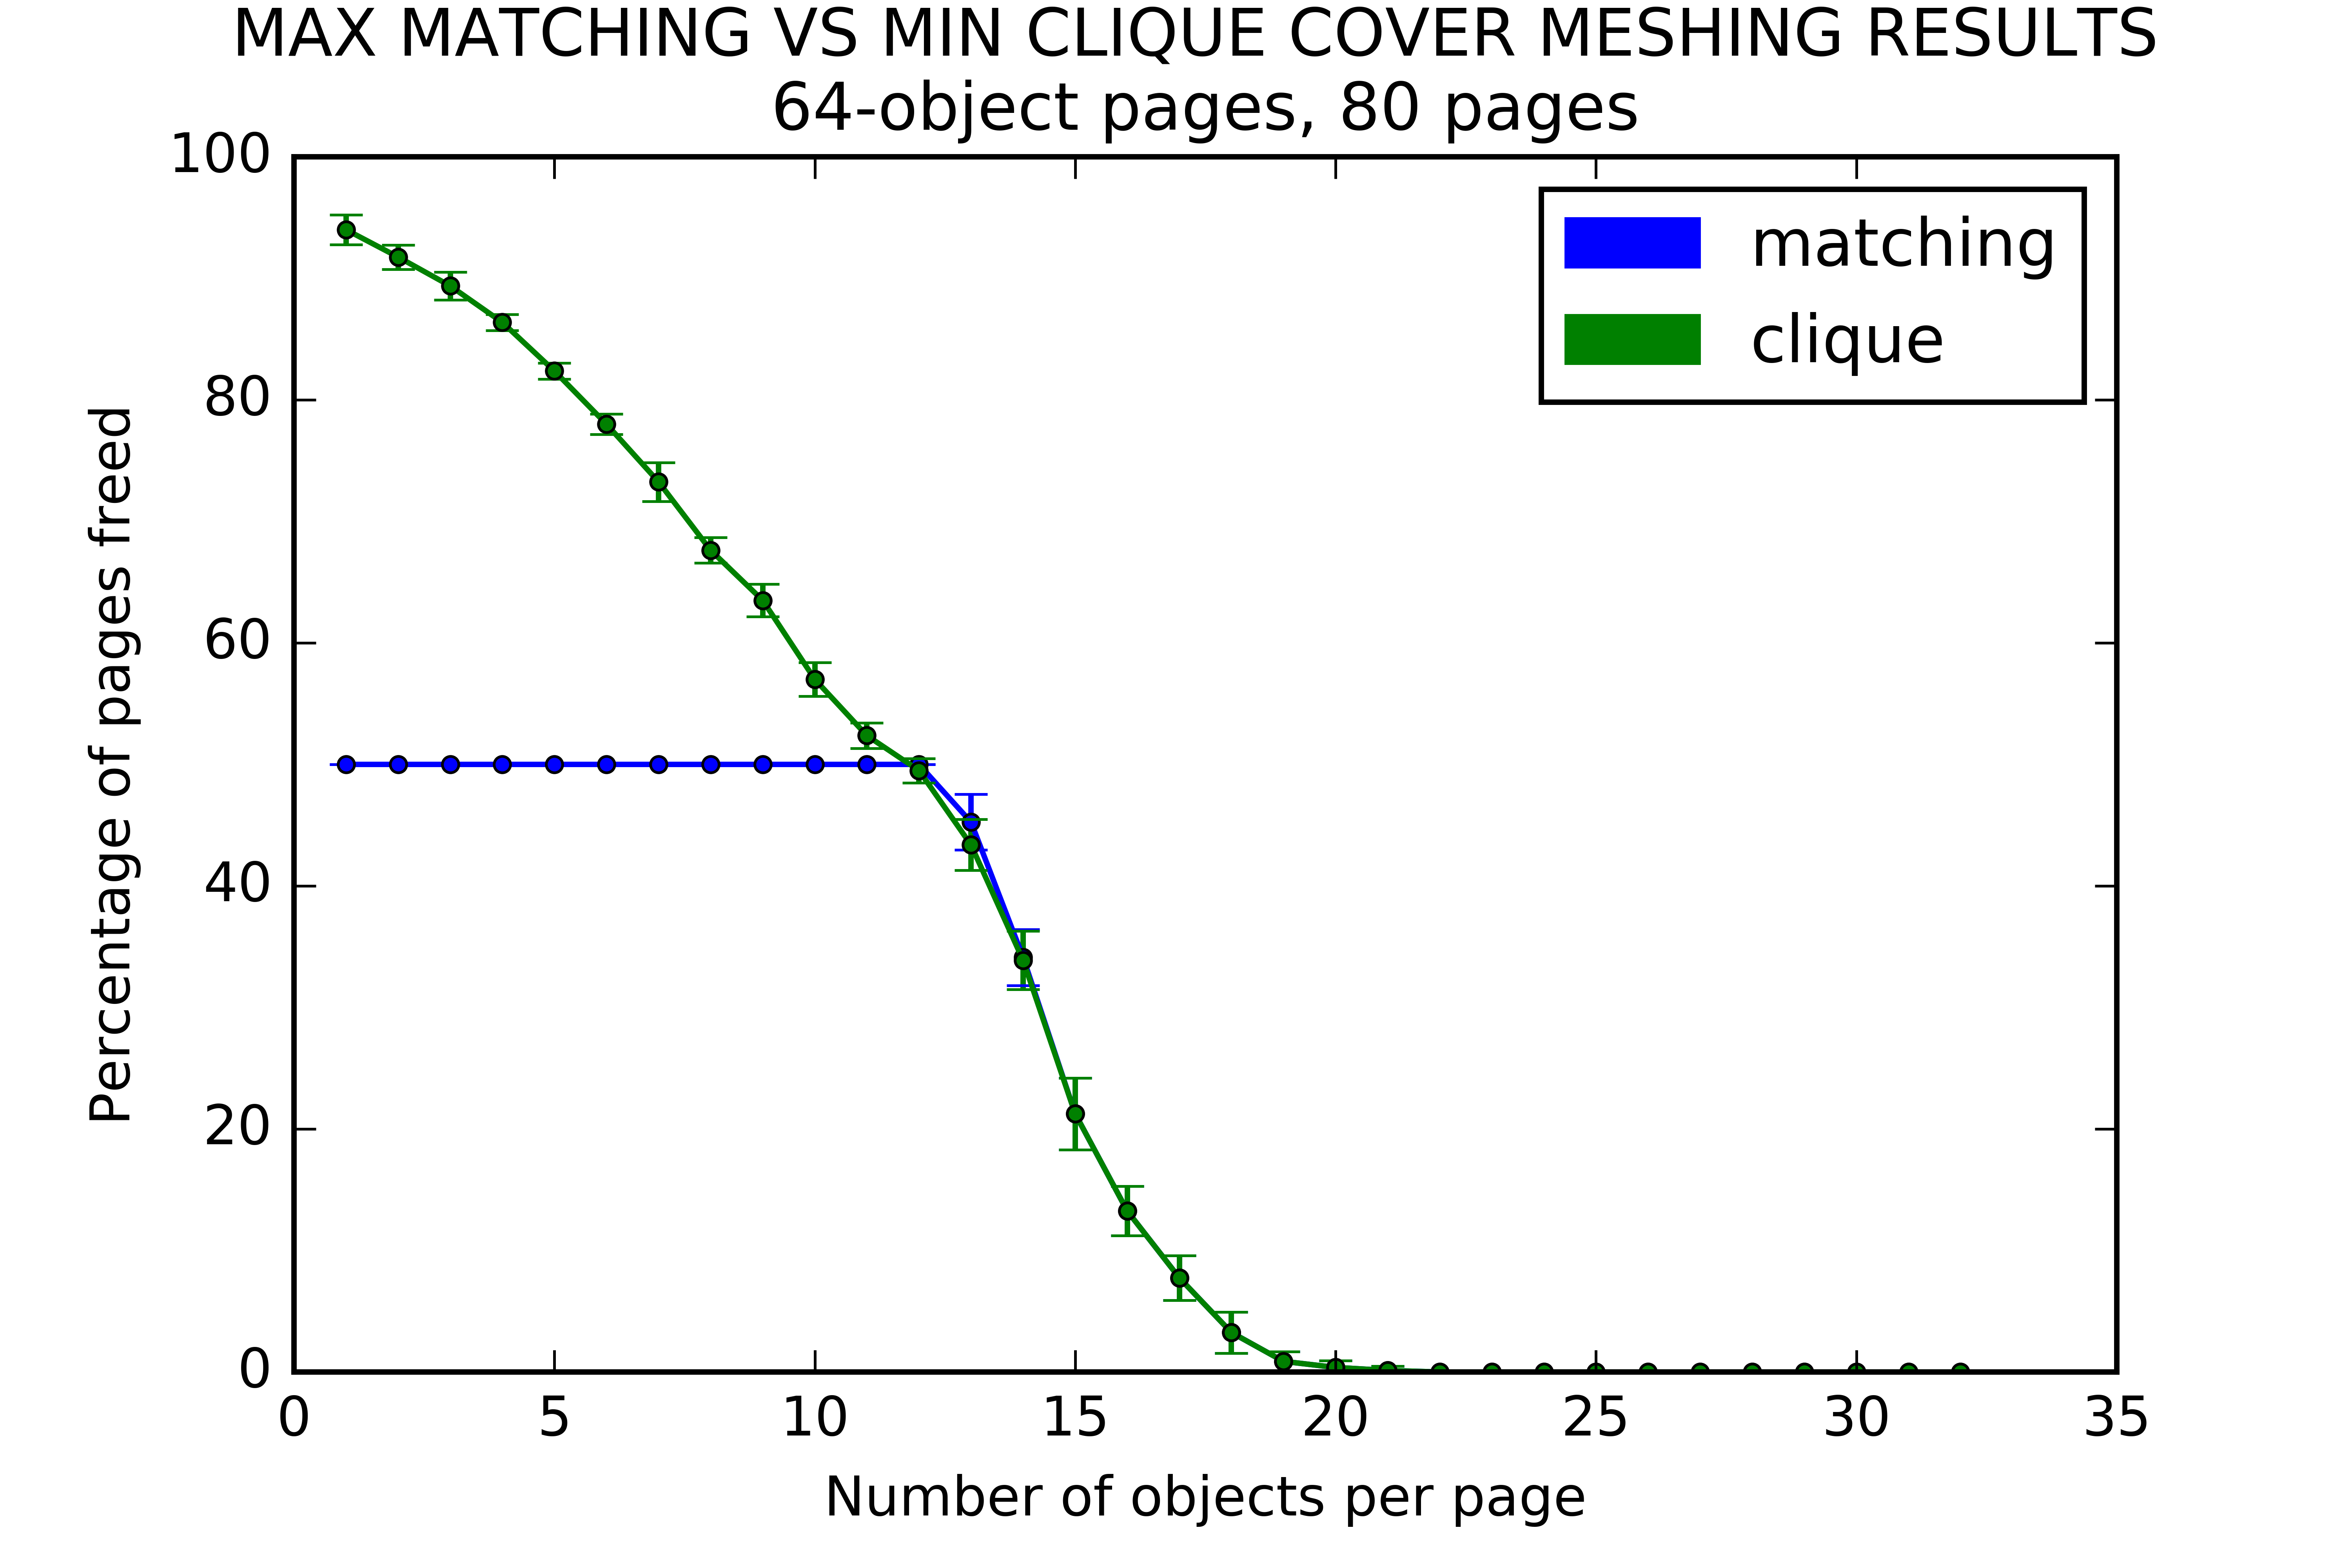
\includegraphics[scale = .5]{figures/64m80ind.png}
\centering
\caption{Average values for max matching and min clique cover on randomly generated graphs.  Graphs were generated from string sets according to the independent bits model; $p = \frac{n}{b}$.  Ten graphs were generated for each occupancy.}
\end{figure}

While constant occupancy graphs are fairly regular, independent bit graphs may not be - since strings have different occupancies, nodes which correspond to strings with relatively low occupancy will tend to have significantly higher degree than other nodes in the graph.  Meanwhile, other nodes may have strings with high occupancy, and therefore only have a few edges (probably with low-occupancy nodes).  So while there are many triangles, when the graph is sparse enough, even meshing cliques of size 3 and 4 will likely "abandon" adjacent high-occupancy nodes, one of which could have been matched with the high degree node to yield the same number of releases.\\
\fi
\iffalse
\subsection{Experimental Comparison}
We might wonder how the maximum matching varies between our two types of random graphs (constant occupancy and independent bits).  To this end, we randomly generated many graphs using both frameworks and determined the size of their maximum matchings.  A summary of the results is displayed below.  Constant occupancy graphs were created by randomly generating strings sets by drawing each string uniformly at random from the set of all length 80 with occupancy $n$.  Independent bit graphs were created by randomly generating string sets by choosing $p$ such that the expected occupancy for each string is equal to $n$, so that the two can be meaningfully compared.


\begin{figure}[h]
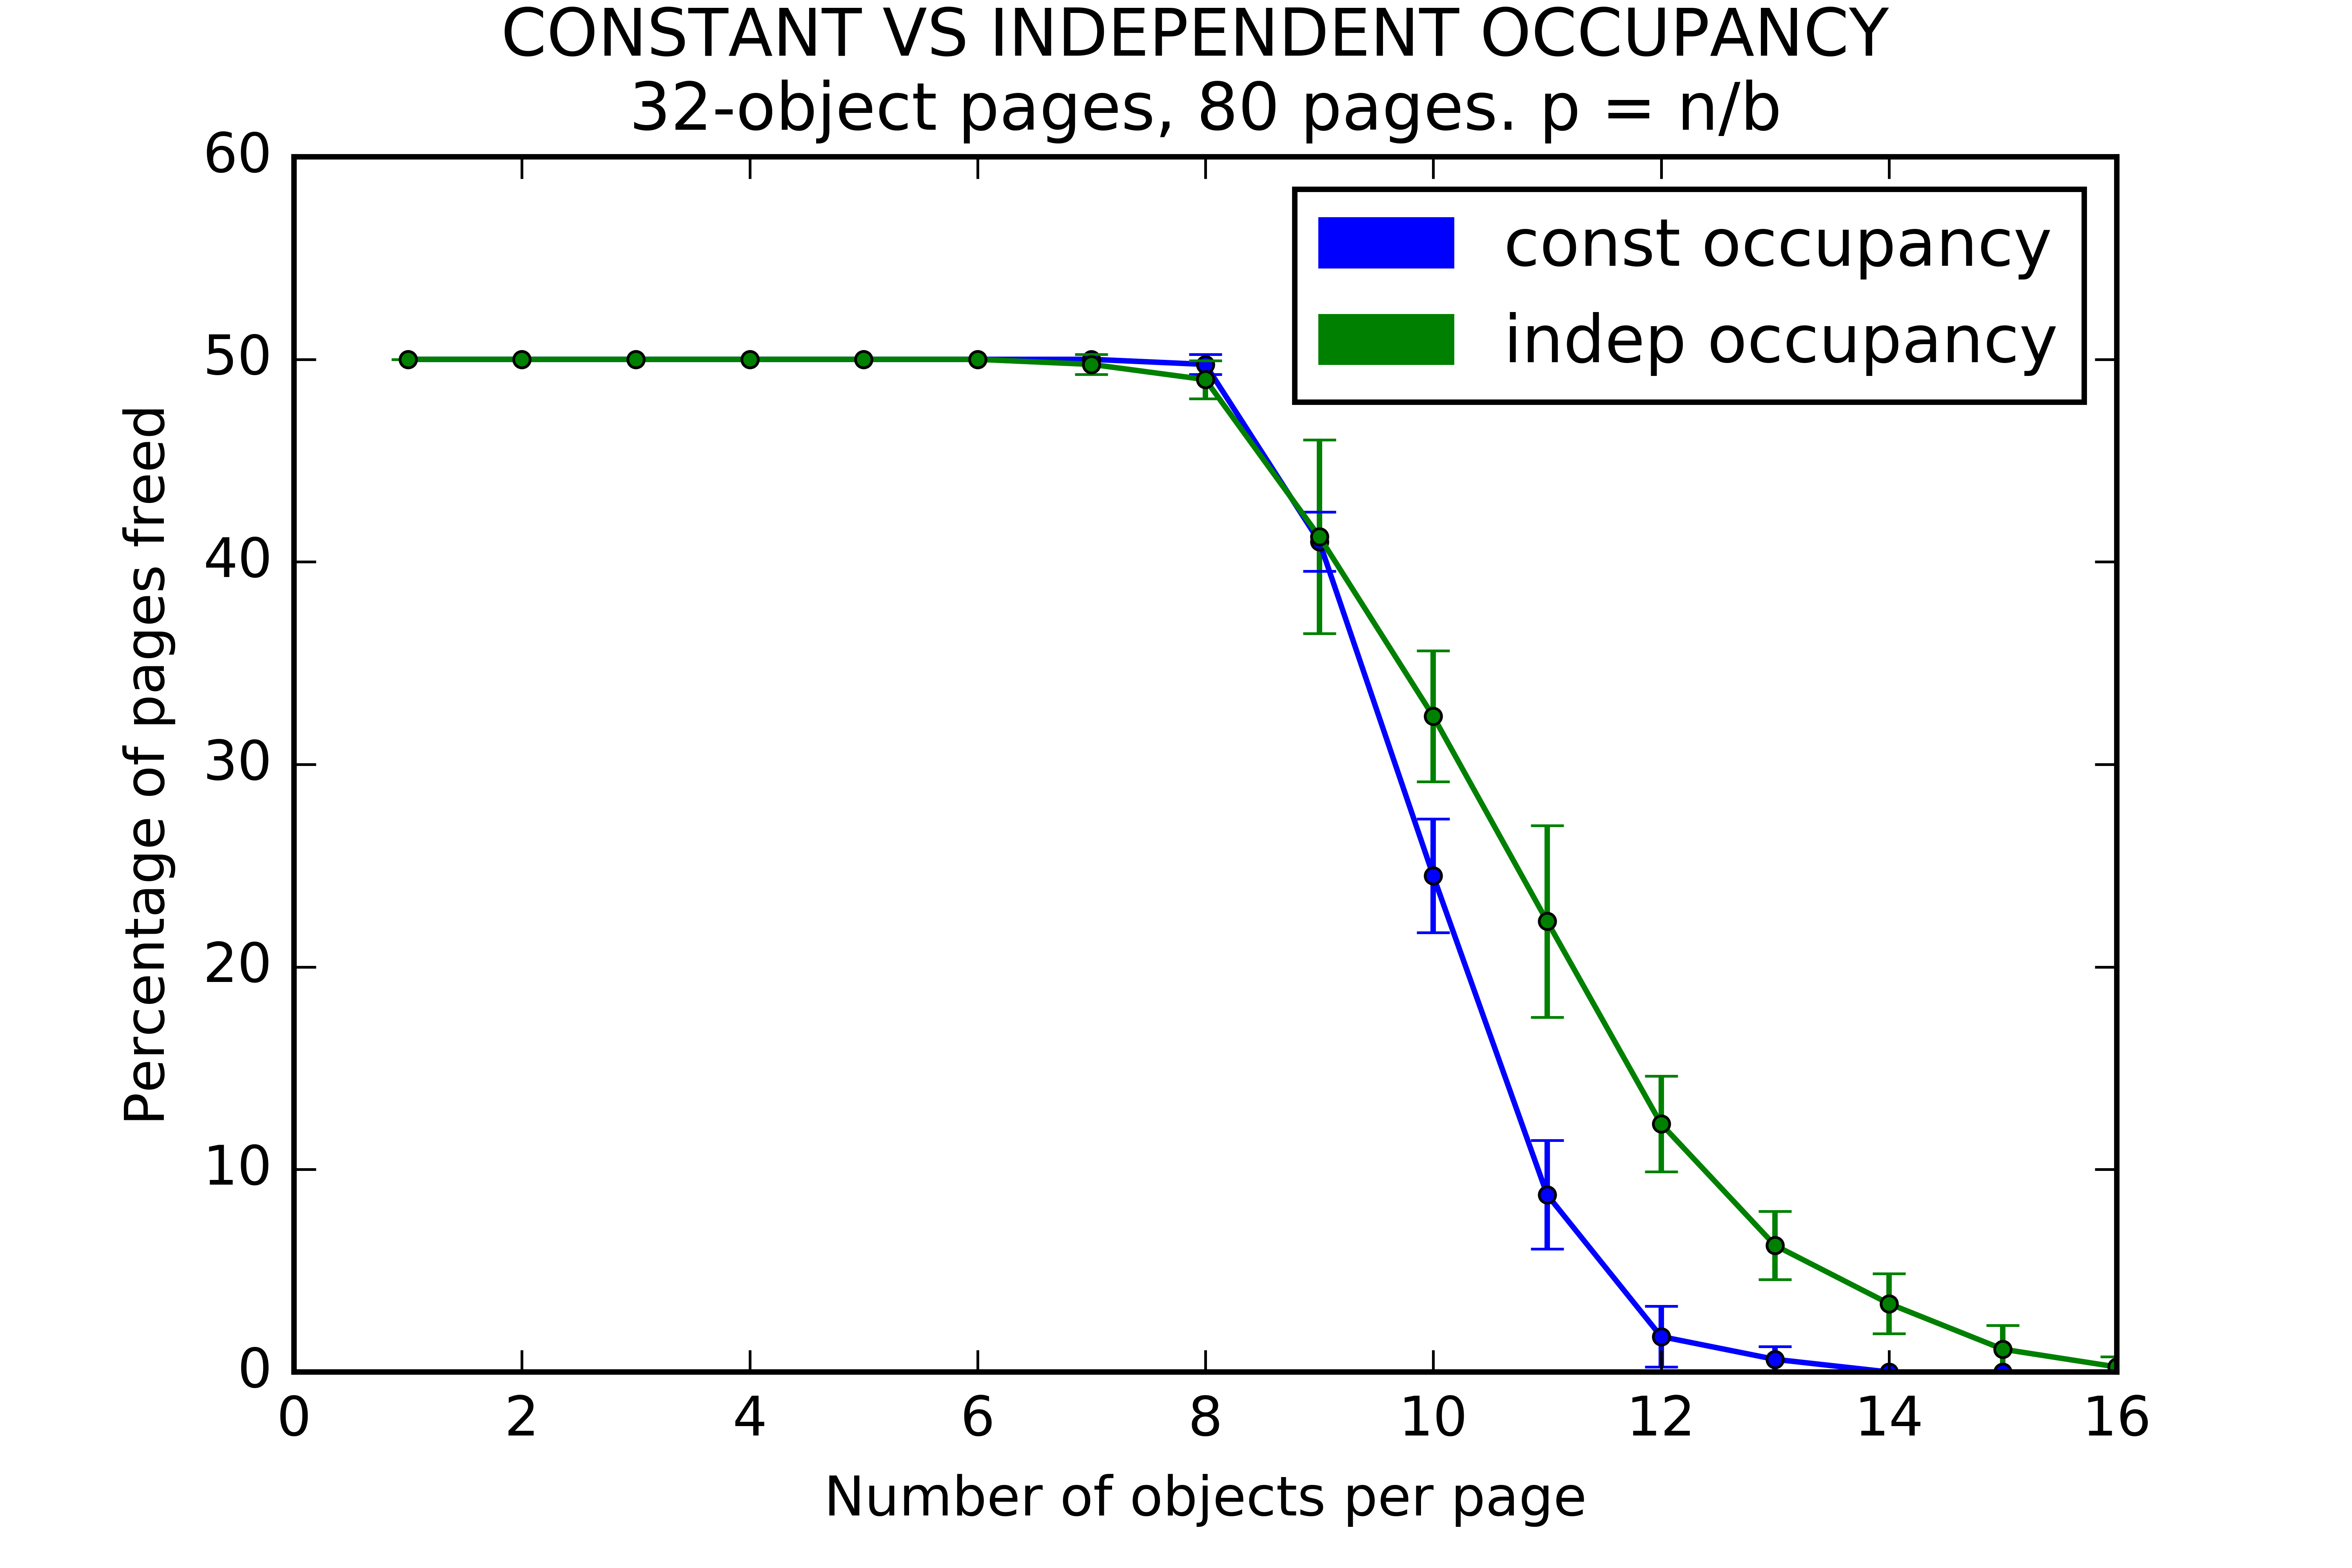
\includegraphics[scale = .5]{figures/constvindep_32,80.png}
\centering
\caption{Average values for max matching on randomly generated constant occupancy and independent bit graphs, $p = \frac{n}{b}$.  Ten graphs were generated for each occupancy.}
\end{figure}

Note that the maximum matching of the independent bit graphs is almost always equal to or larger than the max matching of the respective constant occupancy graphs.  Though we set $p$ so that both types of graphs will have (in expectation) the same occupancy, edges are more common in the independent bits model.
\fi

\iffalse
Assured that solving the maximum matching problem finds a near-optimal meshing with high probability, one might conclude that our engineering task is complete, and that we can simply use existing fast algorithms for maximum matching.  However, due to the fact that meshing occurs during program execution, it is vital that any method used for meshing runs quickly.  In practice, this time constraint prevents use of explicit algorithms for finding a maximum matching on a graph.  Indeed, even constructing a meshing graph from a set of spans is likely to be prohibitively expensive.

We can avoid this computational roadblock by giving up some guarantee of mesh quality.  Specifically, we make use of the classic theorem that any maximal matching on a graph has size at least $1/2$ of the maximum matching on that graph.  Therefore, rather than fully constructing a meshing graph and running a maximum matching algorithm on it, we can instead simply "probe" our span set for pairs of spans that mesh.  When we find such a pair, we greedily mesh it and remove it from the span set.  Finding such a span corresponds to selecting a valid edge in the meshing graph, and including it in the matching without consideration for other details of the graph's structure.  We can continue probing for meshes until we have exhausted all possible remaining meshes in our span set.  At this point we are assured that we have a $1/2$ approximation to the optimal matching (and in practice, we can often expect a much better approximation).


Instead, we test pairs of spans for meshability, meshing any valid pairs we find.  This is equivalent to checking whether a pair of nodes in the graph have an edge, and if so adding it to the matching.  Since we can characterize the probability with which any two spans are meshable, we can argue probabilistically about the size of the matching this procedure will produce.

This idea underpins the design and analysis of \sm.  We argue that we can efficiently approximate this greedy graph procedure without explicitly representing a graph or probing all possible edges.
\fi

\iffalse
The first step in \sm is to random partition the $n$ strings into two sets $S_l$ and $S_r$. It is not hard to show that the size of the maximum matching has decreased by at most a factor 2 in expectation. However, the following lemma (see Appendix for proof) shows that this claim can be significantly strengthened if $nq$ is at least moderately large.

\begin{lemma}
If $nq\geq \Omega(\log n)$ then considering span pairs only between the left and right span sets does not significantly decrease the expected size of the maximum matching.
\end{lemma}
\fi

%Remove or modify following paragraph
\iffalse
Note first that \sm does not consider pairs of spans from the same set.  This is equivalent to removing some edges from the graph before finding a maximal matching, which means that we may fall short of our $1/2$ optimal guarantee.  We are essentially finding a $1/2$ approximation of the maximum matching on a graph with fewer edges.
\fi


\iffalse
We first argue these claims under the assumption that all spans to be meshed have identical occupancies $pb$, and later relax this assumption and show that the claims still hold.  Let $q$ be the probability that two spans with occupancy $pb$ mesh.
\fi

\iffalse

Finally, we must contend with the fact that probes are not independent - a failed probe of two spans is equivalent to discovering that the respective nodes in the meshing graph do not share an edge. In later iterations, when \sm checks a span pair for meshability, we know that those spans are 'connected' by a chain of unmeshable span pairs.  When we learn that two spans are not meshable, it tells us that the spans are similar (if only weakly) since they share at least 1 occupied offset.  A chain of unmeshable spans connecting a span pair therefore weakly suggests that the spans are similar and less likely to mesh.  So in later iterations the actual probability of finding edges decreases.

\begin{conjecture}
An even-length unmeshability cycle in constant occupancy meshing graphs reduces meshing probability q by at most a factor $1- e^{-h}$ for some constant $h$.
\label{conj:depend}
\end{conjecture}
\fi


\iffalse
Let $\node_{i,l}$ denote the node corresponding to the $i$th span in $S_l$, and similarly $\node_{i,r}$ for the node corresponding to the $i$th span in $S_r$.  The expected degree for each node is $q'n/2$ where $q' = (1-p^2)^b$. Each node's degree is between $d$ and $(1+\epsilon)d$ for some $d$, so no node has degree lower than $q'/(1+\epsilon)* n/2$.  So, each edge in this random bipartite graph exists with probability at least $q = q'/(1+\epsilon)$.


Imagine a simplified version of \sm where we only look for meshes for $\node_{1,l}$.  This algorithm tries to mesh it with $t$ nodes $\node_{j,r} \forall j \in [1,1+t]$.  First it is checked against $\node_{1,r}$, and with probability $q$ these nodes have an edge and therefore they mesh.  To mesh with $\node_{1+1,r}$ instead, the first mesh attempt must fail and the second succeed so the probability is $q(1-q)$.  Similarly the probability of finding a mesh with $\node_{1+i,r}$ is $q(1-q)^t$.

Of course, \sm actually checks all nodes $\node_{i,l}$ against $\node_{i+j,r}$ in the jth iteration.  So, for example, to find the probability that $\node_{1,l}$ meshes with $\node_{3,r}$, we must also include the probability that neither $\node_{2,l}$ nor $\node_{3,l}$ mesh with $\node_{3,r}$ (because they were compared to it before $\node_{1,l}$ was).  Each of these two independent events occurs with probability (1-q) so the meshing probability is $q(1-q)^2(1-q)^2$.  More generally, the probability that $\node_{i,l}$ meshes with $\node_{i+j,r}$ is $q(1-q)^{2j}$.

Let $t = k/q$.  Now we can say that the probability $p_{i,l}$ that $\node_{i,l}$ meshes at some point during its $t$ comparisons to nodes in $S_r$ is $$\Pr(u_i \mbox{ has a good match})$$ is
\begin{align*}
r:= q \sum_{i=0}^{k/q-1} \lp 1-q\rp ^{2i} = q \frac{1-(1-q)^{2k/q}}{1-(1-q^2)}
% \geq q \frac{1-e^{-2k}}{2q-q^2}
 > \frac{1-e^{-2k}}{2} \ .
\end{align*}
\fi

\iffalse
Using the union bound over all $Z_j$, we show that the number of meshes found by \sm $Z = \sum_{j \in [1,t]}Z_j$ is less than its expected value $(1-e^{-2k})n/4$ with exponentially low probability.

$$P\lp Z < \lp 1-\epsilon \rp E[Z]\rp \leq \frac{k}{q} \exp\lp - \frac{\epsilon^2\lp 1- e^{-2k}\rp nq}{8k}\rp$$



During the first iteration of the algorithm, we find in expectation $nq/c$ meshes and remove them from the span sets.  In each subsequent iteration, we similarly expect the size of our span sets to decrease by a factor of $q$ as we discover more meshes.  Thus after iteration $i$ we expect our span sets to have size $n/2 \lp 1 - q/c \rp ^{i}$.  Let $t = kc/q$ for some constant k.  Then the expected size of the span sets at the end of the meshing procedure is $n/2 \lp 1 - q/c \rp^{kc/q} \approx n/2 e^{-k}.$
\fi

\iffalse
Note that in the $i$th iteration we expect to make $n/2 \lp 1-q/c\rp ^{i-1}$ probes.  Thus we expect to make $\sum n/2 \lp 1-q/c\rp ^{i-1} = n/2 \lp 1/1-\lp 1-q/c\rp\rp = nc/2q$ probes in total, which is far less than our previous worst-case estimate (which was quadratic).
\fi

\iffalse
\begin{theorem}
Let
\[
w_e=\min\lp \frac{1}{\degree\lp u\rp+1 },\frac{1}{\degree\lp v\rp+1 }\rp
~~\mbox{ and }~~\W=\sum_{e\in E} w_e \ .\]
Then $\W \leq M$.
\label{theorem:lowerbound}
\end{theorem}
\fi

\iffalse
\begin{proof}
%For each edge $e = (u,v) \in G$, define $\W$$(e)=min\lp \frac{1}{\degree\lp u\rp +1},\frac{1}{\degree\lp %v\rp +1}\rp$.  L
Let $U$ be an arbitrary set of $t$ nodes in $G$ where $t$ is odd.   Define $$\W(U) = \sum_{e=(u,v): u,v \in U} w_e \ . $$ As a corollary of Edmonds Matching Polytope Theorem, it can be shown that $\W \leq M$ if  $\W(U) \leq (|U|-1)/2$. We can argue this as follows:


\begin{align*}
\W(U) &= \sum_{(u,v) \in U} \min \left(\frac{1}{\degree(u)+1},\frac{1}{\degree(v)+1}\right )\\
& \leq \sum_{(u,v) \in U}\frac{1}{2}\lp \frac{1}{\degree\lp u \rp +1}+\frac{1}{\degree\lp v\rp +1}\rp\\
&\leq \sum_{(u,v) \in U}\frac{1}{2}\lp \frac{1}{\degree_U\lp u\rp +1}+\frac{1}{\degree_U\lp v\rp +1}\rp\\
&= \frac{1}{2} \sum_{u \in U} \frac{\degree_U\lp u\rp }{\degree_U\lp u\rp +1} \leq  \frac{1}{2} \lp \frac{t-1}{t}\rp  t = \frac{t-1}{2}
\end{align*}
where $\degree_U(u)$ in the number of neighbors of $u$ in the set $U$.
The second line follows from the fact that the minimum of two quantities is bounded above by their average.  The third line follows from the fact that the degree of any node in a subgraph is bounded above by its degree in the original graph.  The fourth line follows from summing over nodes instead of edges, and then reasoning that in the worst case U is a clique and so $\degree_U(u) = t-1$ for all u $u$.
\end{proof}
\fi

\iffalse
See the Appendix for the proof of this theorem. The above bound can be further tightened based on more combinatorial arguments. The proof for the following bound appears in the appendix.
\fi

\iffalse
In some cases, $\W$ is too conservative; it assigns little weight to edges which it could safely have assigned much more.  For example, if $e$ is isolated (meaning its endpoints have degree 1), $\W(e) = \frac{1}{2}$.  However, it is always safe to assign weight 1 to $e$, since $M(G-e) = M(G)-1.\footnote{Here we use M(G) to denote the cardinality of the maximum matching on G.}$  If we modified our rule for $\W$ so that for any edge $e= (u,v)$ s.t. $\degree(u)=\degree(v) = 1$ we assigned weight $ \min(\frac{1}{\degree(u)},\frac{1}{\degree(v)})$ instead of $ \min(\frac{1}{\degree(u)+1},\frac{1}{\degree(v)+1})$, we would always assign weight 1 to isolated edges.

At this point it is natural to ask whether we can remove the $+1$s from the denominator for other edges.  We cannot of course do so for $\degree(u) = \degree(v) = k >1, k \in 2\mathbb{Z}$ since for a clique on k+1 nodes this rule would result in total weight $\frac{k+1}{2}$.\\

However, we can remove the $+1$ under certain circumstances.
\fi
\iffalse
We first show that if one of the endpoints has degree one then this is the case.
%prove several rules of this form.  For each rule we specify values of $\degree(u)$ and $\degree(v)$ for which the %$+1$ can be removed from the denominator of the edge weight.
%First we restate the claim that isolated edges may safely be assigned weight 1.
%\begin{lemma}
%Define $\W(G)$ as follows:\\
%For each $(u,v) \in G$,\\
%if $\degree(u) = \degree(v) = 1$, $\W(u,v) =  \min(\frac{1}{\degree(u)},\frac{1}{\degree(v)})$.\\
%else $\W(u,v) =  \min(\frac{1}{\degree(u)+1},\frac{1}{\degree(v)+1})$.
%Then $\W(G) \leq M(G)$.
%\end{lemma}
%\begin{proof}
%Already proven above.
%\end{proof}
%Next we will amend $\W$ to include the following rule: when one endpoint has degree 1 and the other has %degree k, assign weight $\frac{1}{k}$.

\begin{lemma}
Define $\W(G)$ as follows:\\
For each $(u,v) \in G$,\\
if $\degree(u) = 1$, $\W(u,v) =  \min(\frac{1}{\degree(u)},\frac{1}{\degree(v)})$.\\
else $\W(u,v) =  \min(\frac{1}{\degree(u)+1},\frac{1}{\degree(v)+1})$.

Then $\W(G) \leq M(G)$.
\end{lemma}
\begin{proof}
We have proven that $W(U)\leq \frac{t-1}{2}$ on any odd-size subgraph $U$, $|U| = t$.  Define subsets $U_1$ and $U_2$ of $U$ such that $U_1 \cup U_2 = U$.  $U_1$ is the set of all nodes in $U$ of degree 1 and all nodes in $U$ adjacent to a node of degree 1, and $U_2$ is the set of all other nodes in $U$.  Let $G(U_2)$ denote the subgraph of $U$ induced by $U_2$, and let $|U_1| = x$ where x is even.  Then $W(G(U_2)) = \W(G(U_2)) \leq \frac{t-x-1}{2}$.  So to complete our proof we must show that all remaining edges (call them $E'$) have total weight $\leq \frac{x}{2}$.

Assume WLOG that there are no isolated edges in $G$ (if there are, we can group them with $G(U_2)$ and retain the $\frac{t-x-1}{2}$ bound).

\begin{align*}
\W(E') & \leq \frac{1}{2} \sum_{u,v \in E'} (\frac{1}{\degree(u)}+\frac{1}{\degree(v)})\\
& = \mathlarger{\sum_k} \Big(\sum_{v \in U_1, \degree(v) = k} \frac{\delta}{k} + \frac{k-\delta}{2(k+1)}\Big)
\end{align*}
where $\delta$ denotes the number of degree 1 nodes adjacent to $v$.\\
Let $f(\delta) = \frac{\delta}{k} + \frac{k-\delta}{2(k+1)}$.  We are interested in finding the maximum value $\frac{f(\delta)}{\delta+1}$ can take on; if it can never take a value greater than $\frac{1}{2}$ then $\W(E')$ cannot be greater than $\frac{x}{2}$.

$$\frac{\partial\frac{f(\delta)}{\delta+1}}{\partial \delta} = \frac{2-k}{2k(\delta+1)^2}$$

which is always negative for $k \geq 2$.  Thus $\frac{f(\delta)}{\delta+1}$ is maximized at $\delta = 0$, so  $\frac{f(\delta)}{\delta+1} \leq \frac{k}{2(k+1)} < \frac{1}{2}.$

There is one final detail we have not considered: $x$ might be odd.  In this case, $|U_2|$ is even thus we can't appeal to Theorem 3 to say that $\W(G(U_2)) \leq \frac{t-x-1}{2}$.  However, we can simply remove one node $\node'$ from $U_2$; the resulting odd-size subgraph has weight at most $\frac{t-x-2}{2}$.  Since $\W$ is a valid fractional matching, the weight assigned to all edges adjacent to $\node'$ cannot exceed 1, thus we can say that $\W(G(U_2)) \leq \frac{t-x}{2}$.  Now we must show that $\W(E') \leq \frac{x-1}{2}$.

We have shown that the edge weight per node in $U_1$ cannot exceed $\frac{1}{2}$.  $\W(E')$ is minimized when there is exactly 1 node of degree 1, with a degree k neighbor. In this case, the only edge in $E'$ will be assigned weight $\frac{k}{2(k+1)}<\frac{1}{2}$.  Thus, $\W(E') \leq \frac{1}{2} + \frac{x-2}{2} = \frac{x-1}{2}$ and the lemma is proven.
\end{proof}

Finally, we further amend $\W$ to include the following rule:  when one endpoint has degree 2 and the other degree 3, assign weight $\frac{1}{3}$.
\fi

\iffalse

\begin{lemma}
Define $\W(G)$ as follows:\\
For each $(u,v) \in G$,\\
if $\degree(u) = 1$, or if $\degree(u) = 2$ and $\degree(v) = 3$, $\W(u,v) =  \min(\frac{1}{\degree(u)},\frac{1}{\degree(v)})$.\\
else $\W(u,v) =  \min(\frac{1}{\degree(u)+1},\frac{1}{\degree(v)+1})$.

Then $\W(G) \leq M(G)$.
\end{lemma}
\begin{proof}
See Appendix XXX.
\end{proof}
\fi

\iffalse
One might wonder whether a more general rule can be proven.  So far, the only counterexamples we have presented to W being a lower bound are complete graphs of odd size.  We might try to avoid these failed cases by defining $\W$ so that we include the $+1$ in the denominator only when $\degree(u) = \degree(v) \neq 1$.  In this case, the total weight on a odd-size complete graph is exactly $\frac{t-1}{2}$.

However, this rule gives weight $3(\frac{1}{5}) + 6(\frac{1}{4})$ for a complete graph on five nodes with one edge removed, which is larger than the $\frac{5}{2}$ limit from Edmond's theorem.  So this rule does not produce a valid lower bound for maximum matching.

Currently we are hoping to determine whether the following conjecture is true:
\begin{conjecture}
Define $\W(G)$ as follows:\\
For each $(u,v) \in G$,\\
if $|\degree(u) - \degree(v)|\leq 1$,$\W(u,v) =  \min(\frac{1}{\degree(u)+1},\frac{1}{\degree(v)+1})$.\\
else $\W(u,v) =  \min(\frac{1}{\degree(u)},\frac{1}{\degree(v)})$.

Then $\W(G) \leq M(G)$.
\end{conjecture}
\fi

\iffalse
\paragraph{Estimating $\W$}
One of the main features of our estimate $\W$ is that the expected size of $\W$ can be relatively easily estimated in meshing graphs. Specifically, let $p$ be the probability that two pages mesh. Let given two pages $u$ and $v$, the expected value of $w_e=(1/(\max(\degree(u),\degree(v))+1))$
\fi





disadvantage of the Applications written in these languages can suffer from
Because heap-allocated objects in C and C++ cannot be relocated,
memory allocators for these languages can introduce heap
fragmentation. Existing techniques like segregated-fit allocators
reduce fragmentation compared to alternatives, but they can not
eliminate it, especially under adversarial or worst-case
workloads. Managed languages minimize fragmentation through compacting
garbage collection, where live objects are relocated adjacent to each
other and free space is returned to the operating system.




virtual pages to point to the same physical page, we mesh objects on
those pages provided their virtual offsets do not overlap. This allows
us to store objects from several virtual pages on a single physical
page, freeing the other physical pages and increasing usable memory.

We present a suite of practical algorithms for memory compaction
through meshing, and develop new theoretical results which guide the
design of these algorithms and probabilistically guarantee their
efficacy.  We implement a meshing memory allocater as a Linux shared
library, libmesh, that works with unmodified C and C++ programs.  We
show that meshing introduces low time overhead in practice, and is
able to reduce memory usage by XX percent over a set of representative
benchmarks.


Given such an adversarial
environment, a runtime system can not guarantee that it can identify
all allocation references at any given point in time.  Without
precisely identifying \textit{all} references, allocations can not
safely be relocated, as all locations that point to a moved allocation
need to be updated for the program to continue executing correctly.

Because objects can not be relocated, memory allocators for these
languages can not perform compaction and thus programs may suffer from
fragmentation.  Fragmentation is a result of the fact that while a
user's program manages memory at the granularity of \textit{bytes},
operating systems manage memory at the level of \textit{pages} (4 KiB
on most contemporary architectures).  Fragmentation occurs when a
small number of program objects require the reservation of a
corresponding large number of pages from the operating system.
Fragmentation can result in a program requiring orders of magnitude
more memory from the operating system than is required by the
semantics of the program.


Fragmentation has been widely
studied~\cite{johnstone:1998:fragmentation} and solved for managed
languages with \textit{moving
  compaction}~\cite{hansen:1969:compaction,fenichel:1969:compaction}
in the late 1960s.  Compaction minimizes fragmentation by moving live
objects close together.  Contemporary runtimes like the Hotspot
JVM~\cite{microystems2006memory}, The .NET
VM~\cite{microsoft:dotnet-gc}, the SpiderMonkey JavaScript
VM~\cite{mozilla:spidermonkey-compaction} and others implement moving
compaction as part of their garbage collection algorithms.



%The rest of this paper is organized as follows. Section~ introduces the concept of meshing and show how our approach reduces fragmentation in a representative unmanaged program. 
%Section~\ref{sec:allocator} details \Mesh's efficient memory
%allocator.  Section~\ref{sec:theory} presents the theoretical results
%that make meshing efficient and
%practical. Section~\ref{sec:evaluation} provides an empirical evaluation of \Mesh, and section~\ref{sec:discussion} discusses how
%several classes of applications would benefit from deeper integration
%with \Mesh.  Finally, section~\ref{sec:related-work} discusses related
%work, and section~\ref{sec:conclusion} concludes this paper.


%% TODO: pull out Redis discussion. Just an overview of meshing.
%% TODO: meshing algorithms, meshing analysis, meshing implementation

\section{Meshing Overview}
\label{sec:meshing}

\begin{comment}
  \begin{figure}[!t]
\centering
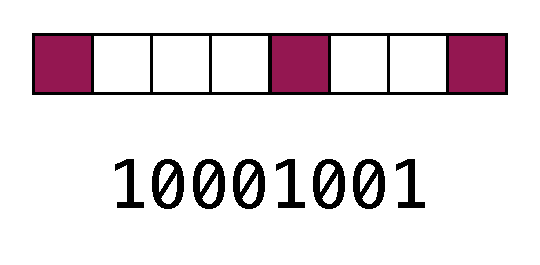
\includegraphics[width=.3\textwidth]{figures/bitmap_bitstring}
\caption{The bitmaps managing the allocated space in a span
  (visualized as allocated objects in the span, top) can be
  represented as bitstrings of 0s and 1s (bottom), where a 1
  corresponds to an allocated object and 0 to free space.}
\label{fig:bitmap-bitstring}
\end{figure}
\end{comment}

To give an intuition for how \mesh works, why it is dependable, and
when it shines, we walk through how \mesh manages memory for a
representative application, Redis.

%% Redis is a data structure server that operates primarily in memory.  It is high performance, written in C.
%% Not just a key value store, also channels, change notifications, sets...  Often sees steady writes over time.
%% Redis devs have seen memory fragmentation as an issue.
%% Implemented a custom defrag scheme.

%% High level things to hit:
%% - redis bg
%% - redis workload: moderate heap footprint, lots of writes (LRU?)
%% - what is fragmentation
%% - state of the practice: custom best effort defrag
%% - mesh: meshing
%% - mesh: allocations and frees (randomness, reasoning in expectation, worst case)
%% - mesh: finding meshes
%% - mesh: convergence over time
%% - mesh: implicit (free path) vs explicit API call

\subsection{Redis}

Redis is an ``in-memory data structure store'' and is used in a
variety of roles.  It can act as a database and document store,
supporting simple lookup and indexing operations.  Redis performs
admirably as a cache, with built-in mechanisms to expire data.
Additionally, it can act as a message broker with publish and
subscribe operations.

Redis aims to be reliable and, above all, fast.  It is implemented in C
with a single-threaded event loop built on top of non-blocking IO.
Operations performed on behalf of clients complete without touching
disk.

Redis often has both a significant heap footprint (storing or caching
data), and a steady stream of writes.
% (it doesn't necessarily have a
%write-heavy `load' then read-heavy `serve' phase shift).

\subsubsection{Fragmentation}


\begin{figure}[!t]
  \centering
  \begin{subfigure}[t]{.5\textwidth}
    \centering
    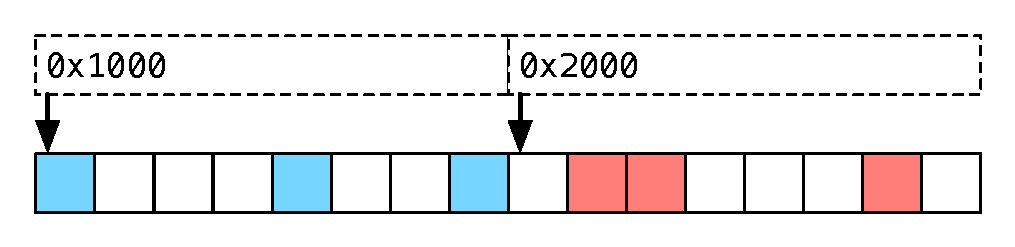
\includegraphics[width=\textwidth]{figures/before_meshing}
    \caption{Two adjacent spans that are candidates for meshing.}
  \end{subfigure}%
  ~

  \begin{subfigure}[t]{.5\textwidth}
    \centering
    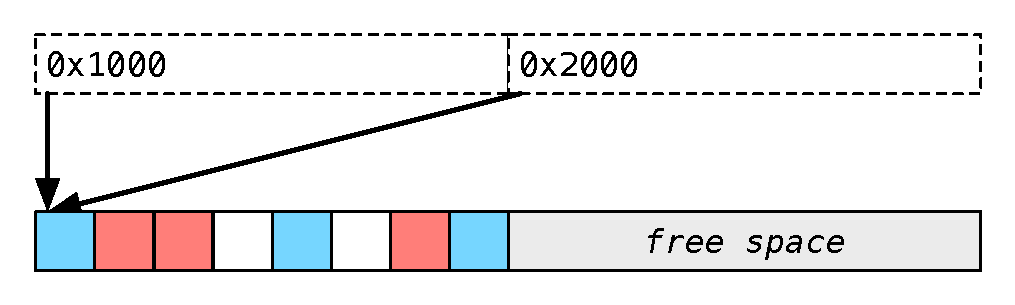
\includegraphics[width=\textwidth]{figures/after_meshing}
    \caption{After meshing, both virtual spans refer to the same
      physical \newline span, with live objects interleaved.}
  \end{subfigure}
  \caption{Virtual and physical memory layout before and after
    meshing.  After meshing, physical span occupancy has increased
    from 37.5\% to 75\% and one physical span has been returned to the
    OS for reuse.}
  \label{fig:meshing}
\end{figure}


Memory fragmentation, introduced in Section~\ref{sec:introduction},
occurs when the ratio of program-allocated memory to operating-system
reserved memory becomes high:

\begin{align*}
\text{Fragmentation} = \frac{\text{Reserved}}{\text{Allocated}}
\end{align*}

\textit{XXX: I think it is worth noting that an allocator that stored
  a very high amount of metadata per allocation (e.g. tracking the
  meshability graph explicitly) would be indistinguishable from a
  highly-fragmented allocator from the perspective of the OS.  Not
  sure how to work that in.}

%% Informally, fragmentation occurs because the application manages
%% memory in bytes, while the operating system manages memory at page
%% granularity -- 4 KiB on most current architectures.  Sparsely allocated
%% application addresses ``pin down'' otherwise vacant OS pages.

%% Many managed languages like Java and JavaScript do not experience
%% memory fragmentation due to the combination of language soundness and
%% garbage collection implementations.  Languages are designed in such a
%% way that implementations can enumerate and update all object
%% references, enabling garbage collectors to periodically compact live
%% objects.  This isn't possible for unmanaged languages like C, C++ and
%% Rust, as it is not possible to soundly enumerate all object
%% references.

Redis users experience memory fragmentation as a significant problem
in real-world deployments.  To address this, Redis developers have
implemented an application-level defragmentation scheme.
\textit{(XXX: describe defragmentation)}.  This is unprincipled and
best-effort, but solves a big enough problem and works well enough
that it ships in the default build of Redis.

\subsection{Meshing}

Meshing minimizes fragmentation in real-world applications like Redis,
providing compaction without requiring updates to allocated virtual
addresses.  A key insight of \mesh is that virtual address space is
effectively free while physical memory is a scarce resource.

Figure~\ref{fig:meshing} illustrates the meshing process.  Two
\textit{spans} of memory are shown that have low utilization, each is
under $40\%$ occupied.  Importantly for meshing, these spans contain
allocations with non-overlapping offsets counting at zero from the
start of each span.  More formally, we can say that $t$ spans
\textit{\mesh} if and only if the sum of each offset across the $t$
spans sum to 1 or less:

\begin{align}
  \forall k \in [0, b-1]. \sum_{0 \leq i \leq t} s_i[k] \leq 1
\end{align}

where $b$ is span length, and $s_i[k] = 1$ iff there is an object at the $k$th offset of span i.

Meshing consolidates allocations from each onto one physical span.
Each object in the resulting meshed span resides at the same offset as
it did in its original span.  The virtual-to-physical mapping for the
process is updated so that both virtual spans point at the same
physical span, and the second physical span can be returned to the OS
or used for subsequent allocations.  More than two spans can be meshed this way, in which case all objects are consolidated to a single span and all other spans can be reused.


\subsubsection{Allocation, Randomness and Worst-Case}

Meshing introduces a limited amount of randomness to ensure that we
can reason about meshing spans in expectation.

We want to avoid the situation where all spans have low occupancy but
are non-meshable.  In the most extreme case, each span could have exactly 1 object, with all objects residing at the same offset.  In this case the system exhibits maximum fragmentation and no meshing is possible.  

To minimize the chance of such unrecoverable fragmentation, during allocation Mesh allocates each object uniformly at random among the available offsets in the target span.  As a result, the probability of the worst case scenario above is very low:

$$P(\textit{all objects at same offset}) = (\frac{1}{b})^{k-1}$$

where k is the number of spans.

We use this randomness to prove more robust guarantees of Mesh's performance in Section ~\ref{sec:theory} and to guide our design of meshing algorithms presented in Section XXX.

\textit{XXX: should insert a treatment of Emery's ideas about address obliviousness here.}


\subsubsection{Finding Meshes}

Given a set of spans, we would like if possible to mesh them so as to free as many spans as possible for other uses.  We can think of this task as that of partitioning the spans into subsets such that the spans in each subset mesh.  An optimal partition would minimize the number of such subsets.

In Section ~\ref{sec:theory} we discuss how finding the optimal meshing is not feasible, and argue that a solving a simplified version of the problem is usually good enough.  In section XXX we present practical methods for finding high-quality meshes under real-world time constraints.


%% XXX: we should unify talking about ``objects'' and ``allocations''
%% -- allocations is probably better for unmanaged languages where
%% objects have a specific interpretation.

%% Meshing works on \textit{spans} -- contiguous regions of memory where
%% the size of a span is a multiple of the page size between 4 KiB and
%% 128 KiB.  Each span allocates objects of a single-size only, for
%% example a 4 KiB span might hold 32 objects of size 128 bytes.  We can
%% represent a span by a \textit{bitstring}, as in
%% Figure~\ref{fig:bitmap-bitstring}, a string with a 1 for an allocated
%% object at that offset from the start of the span and 0 otherwise.  The
%% length of the bitstring is the number of objects that span holds.

%% This definition characterizes the constraints of the technique by
%% which meshing is possible, wherein two or more spans are meshed or
%% "stacked" on top of each other.  

%% The layout and management of a program's heap guide how we consider
%% meshing.  In a running program, the heap is managed as a number of
%% different \textit{size classes} along with a region consisting of
%% large allocations.  Allocations are fulfilled from the smallest size
%% class they fit in (e.g. an allocation request for 50 bytes is
%% satisfied by the 64-byte size class), and objects larger than 16 KiB
%% are individually served from the large allocation region.

%% We treat each size class as an independent instance of the meshing
%% problem, and large allocations are not meshed.  As large allocations
%% are all many multiples of the page size significant fragmentation
%% between them does not exist.  The number of size-classes is fixed at
%% compilation time and constant during the execution of a program.

%% From here, we consider meshing as dealing with a single size-class,
%% and refer to all spans within this size class as $S$.  If we want to
%% mesh the entire heap, this means solving $n$ instances of the meshing
%% problem, where $n$ is the number of size classes.


%% Finally, meshing relies on the fact that there are two types of spans,
%% virtual and physical.  A \textit{virtual} span refers to the memory
%% addresses visible to the program being executed, while a
%% \textit{physical} span corresponds to the area in memory where
%% allocated objects live.  Meshing is concerned with minimizing the
%% count of in-use physical spans without modifying or moving virtual
%% spans.  As noted in Section~\ref{sec:introduction}, we cannot change
%% or modify virtual addresses returned from the allocator, as we do not
%% have a way to enumerate and update all references the program has
%% stored.  Since the last two digits of a virtual address directly
%% specify the offset of the referenced object in the span, objects
%% cannot be safely relocated to a different offset, leading to our

%% Allocated objects and free space within a span are tracked by the
%% memory allocator as a bitmap (see Section~\ref{sec:allocator}) -- the
%% in-memory representation of a bitstring.  For example, for objects of
%% size 32 and a span size of 4 KiB, the span can hold 128 32-byte
%% objects, so allocated objects are be tracked with a 128-bit bitmap.
%% Each allocated object in a running program has a unique
%% \textit{(bitmap, offset)} tuple.  Bitmaps are between 8 and 256-bits
%% in length.

%% We can therefore think of the meshing problem as that of partitioning
%% a set of equal-length bitstrings such that the bitstrings in each subset
%% mesh.  An optimal partition would minimize the number of such subsets.
%% This abstraction allows us to analyze the complexity of this computational
%% task in Section~\ref{sec:theory}.
